\section{Introduction}
\label{sec:introduction}

Division of Labor is known as  an essential factor for achieving wealth of human beings. In division of labor, individuals and organizations acquire specialised capabilities and play different roles in a system, and either form combinations or trade to take advantage of  their and others' capabilities. 

In the recent years, more and more information on tasks is being circulated on the Internet, and there are many labor resources accessible through it. This allows us to take the computational approach to division of labor, in which AI and algorithm agents assign appropriate tasks to workers to achieve specific goals.
There are many studies that address topics related to division of labor. 
For example, many papers on crowdsourcing address algorithms  for task assignment considering given objective functions, such as price and required time.
However, division of labor is different from  just ``decomposing into microtasks.'' Task decomposition itself does not necessary cause division of labor, if we obtain a set of tasks each of which requires workers to have the same set of capabilities represented by  their attributes (such as skills and locations of workers).
We need {\it task classes} that require different capabilities and {\it worker classes} that have workers with different capabilities.
For example, assume that we have a set of sentences in English that needs to be translated into Braille in Japanese. 
Decomposing into a set of tasks each of which translates one sentence into Braille does not cause a division of labor, because we have only one task class that require the same skills.
In contrast, decomposing them into a set of translation tasks from English to Japanese and another set of translation tasks from Japanese into Japanese Braille result in division of labor; then we have two task classes that require different specialized capabilities for translation.
In addition, we may be able to further decompose the obtained task classes. For example, we can find a {\it subclass} under the English-Japanese translation task class in which the sentences require detailed knowledge of a particular domain (e.g., Japanese pop stars). 
Then, workers who have the knowledge can be assigned to the tasks in the subclass.
Note that how to decompose task classes depends on the availability of workers in the worker pool. If we had a lot of people who are good at translating English Braille into Japanese Braille, we would have different subclasses: Translating English into Braille and translating it into Japanese one.
 

Adam Smith pointed out that the efficiency of division of labor comes from the following benefits: Increase of workers' capabilities, lower switching cost of tasks, and machines taking place of manual labor \cite{Smi76}. 
Taking different roles and trading or combining their abilities and products has a dramatic effect; it would be impossible for us to obtain many things today, let's say a smartphone, in exchange for the work for several to tens of hours, if each of us made our smartphone ourselves, without having a large amount of people who produce materials and semiconductor chips, design the electronic circuit and user interface, develop software, etc.
Computational division of labor will be one of the important issues in Future of Work \cite{Sih+20}.
However, as we will show, this area is still in its infancy and there are a lot of things we can do.
%We note that there are still   a lot of things we can do from the division of labor perspective.
%the computational approach to division of labor.
%division of labor  Division of Labor provides criterion on what will be good assignments for our society.

\begin{figure}[t]
\centering
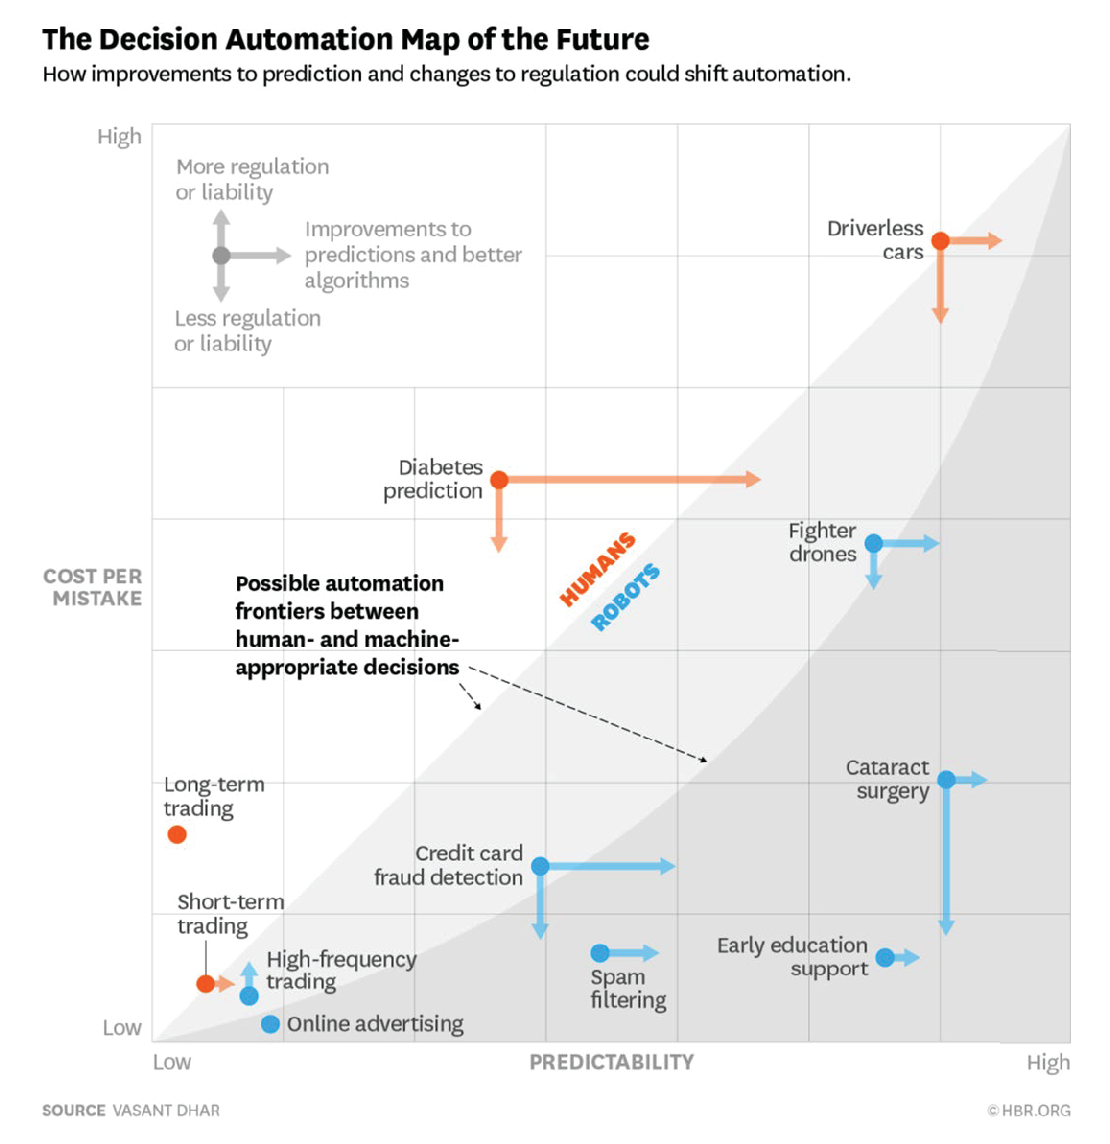
\includegraphics[width=100mm]{submissions_new/morishima/figures/decision-automation-map.eps}
\label{fig:decisions}
\caption{Whether decisions in particular areas should be made by humans or AI \cite{Dha16}. The x-axis is the predictability by AI. The y-axis is the cost per mistake.
This figure states that decisions can be made by AI if it has high predictability and low cost per mistake. We already have many things for which we can use AI (dots) and we expect to have more things as we have
improvement in predictions and algorithms (horizontal arrows), and regulations or liability changes (vertical arrows) in the near future.}
\end{figure}


While we have an environment that makes us ready to pursue the computational division of labor today, there is the demand for the computational approach.
We recently noticed that worker availability can be changed in a disease pandemic. However, one of the most important factors is the rapid growth of AI. Figure \ref{fig:decisions} shows whether decisions in particular areas should be performed by humans or AIs at present and the potential changes in the near future. 
It depends not only  the predictability but also cost per mistake. As shown in the figure, we already have a lot of things we can rely on  AI, and there will be more and more in the near future, as we see 
%As shown in the figure, the results are affected by many factors that change rapidly today, such as
improvement to predictions and better algorithms, and regulations or liability changes. 
%t is certain that more and more tasks are taken by AI nowadays and 
Many new kinds of commercial services that employ new combinations of AI and human resources are emerging at a great speed.
This means that AI is important not only for implementing solutions of computational division of labor, but also as  {\it AI workers}, that work in collaboration with human workers.
In addition, the change spreads world wide in a short period of time; we see accelerating technology change \cite{Kur01} and new services and industries are deployed at a large scale internationally.
Such a {\it scale} and {\it speed} of change caused by the {\it rapid growth of AI technology} requires the computational approach to the division of labor problems.

Note that there are a variety of tasks beyond decision tasks, which often require other capabilities than high predictability such as flexible response, some of which are difficult for the AI today, although the situation may change in the near future.
%Note that predictability and cost per mistake are not the only factors to decide whether the task should be done by human or AI workers. 
For example, think about a conveyor belt sushi restaurant which is popular in Japan. Although making oval-shaped rices for sushi used to be considered as an expert task that is allowed to be performed by  experienced staff members only, the advance of technology allowed
machines to make the rices in conveyor belt sushi restaurants. Even fish slices to be put onto the rice are being made by machines with AI.
%This does not mean that they do not need human workers.
However, there are many other tasks that are being performed by humans workers. They {\it develop} and {\it teach} AI,  communicate with customers,  cook special kinds of sushi, and deal with non-routine issues, all of which are difficult tasks for AI today.


\eat{
However, this does not mean that humans are responsible for difficult tasks. Machines become gradually smart enough to be responsible for difficult tasks that used to be performed by only experts if it is a fixed form task, because the cost to hire experts is expensive. 
For example, think about a conveyor belt sushi restaurant which is popular in Japan. In traditional sushi restaurants, making oval-shaped rices are considered to be an expert task that are allowed to be performed by  experienced staff members only.
However, in conveyor belt sushi restaurant, machines make the rices. Even fish slices to be put onto the rice are being made by machines. 
Then, what human workers do? They are putting the fish slices onto the rice and then put them onto the belt conveyor. There are a large number of items in the menu that often changes, and it is difficult for machines to deal with the small changeable things.
Although putting the fish slices are not expert tasks, it is a task that require humans' flexibility.  Actually, most of restaurant staffs are part-time workers in conveyor belt sushi restaurant.
}


%In addition, the change spreads world wide in a short period of time. 

%In order to cope with the speed and scale at the world scale , and AIs are expected to be able to perform more and more tasks in the near future.





\eat{
\begin{itemize}
    \item Scale
    \item Speed
    \item AI
\end{itemize}
}

In this article, we investigate problems on computational division of labor and look at the current status of research on crowdsourcing and human-in-the-loop systems on the Internet from the division-of-labor perspective.
We chose these areas because in the near future, we expect that many jobs will be supplied by human-in-the-loop online job platforms \cite{GMT+19}.

\textbf{Paper Outline.}
The rest of the paper is organized as follows.
In Section~\ref{sec:computationaldivisionoflabor},
we explain what computational division of labor problems deal with and introduce a set of dimensions and terms to classify existing solutions for problems related to
computational division of labor.
In Section~\ref{sec:relatedstatus}, we look into some of existing literature and investigate the current status.
Section \ref{sec:challenges} discusses  challenges and open problems. 



\section{Computational Division of Labor}
\label{sec:computationaldivisionoflabor}


\begin{figure}[t]
    \centering
    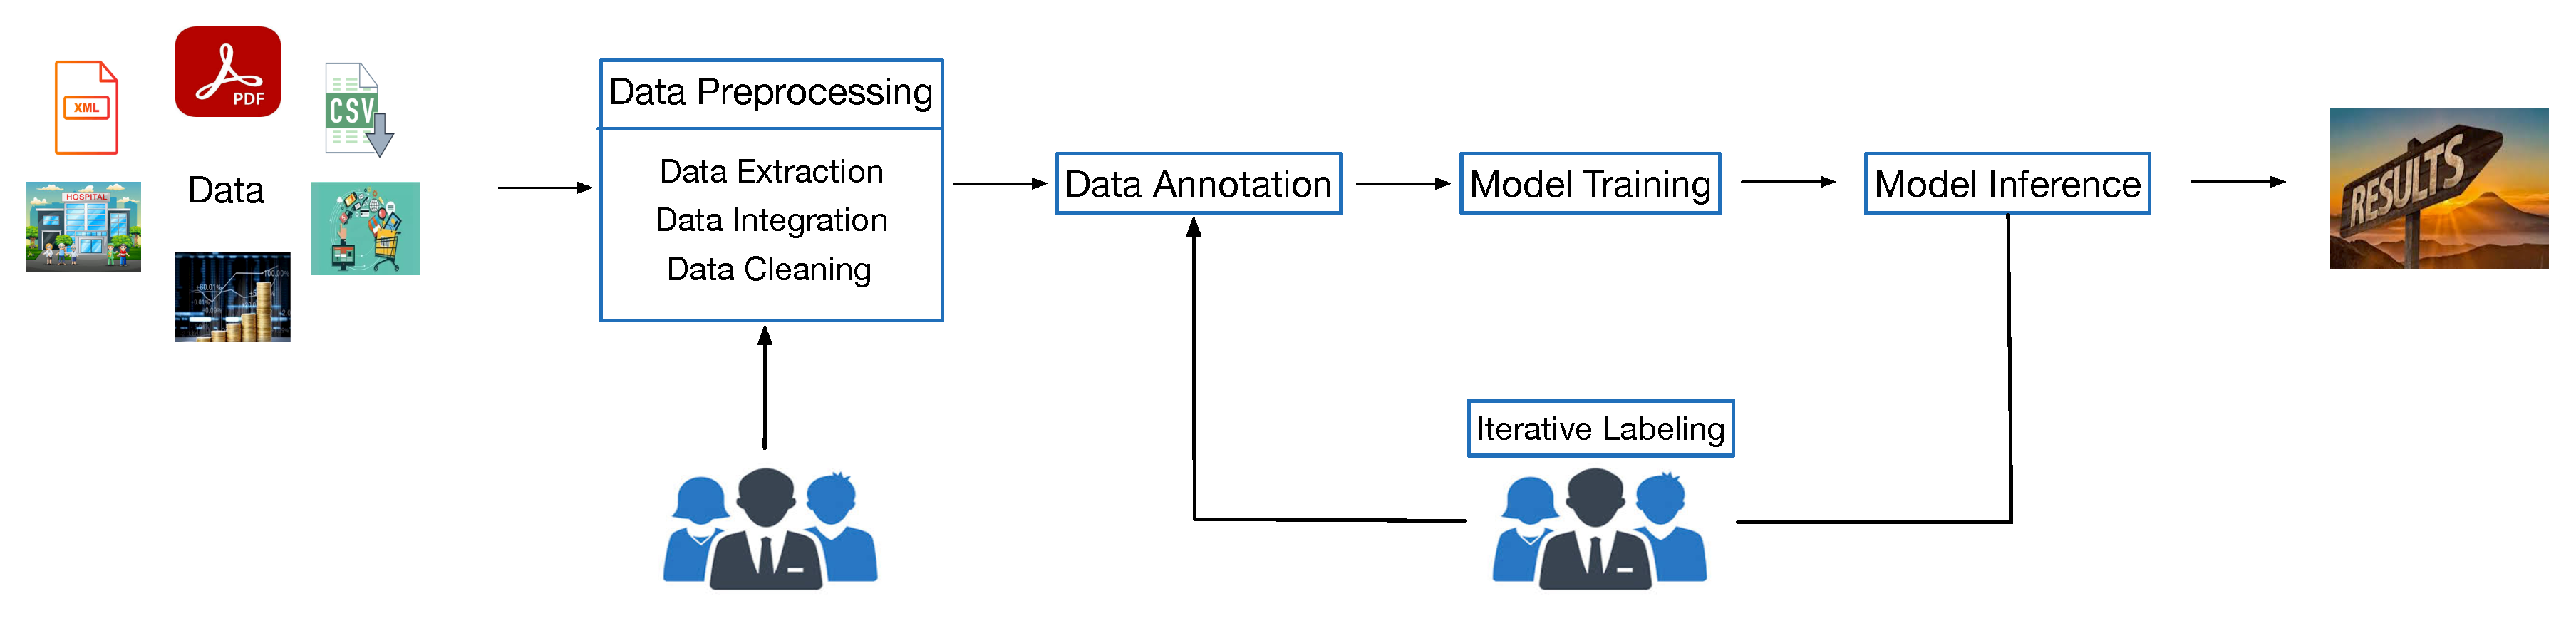
\includegraphics[width=100mm]{submissions_new/morishima/figures/framework.eps}
    \caption{Framework for computational division of labor}
    \label{fig:framework}
\end{figure}

\begin{figure}[t]
    \centering
    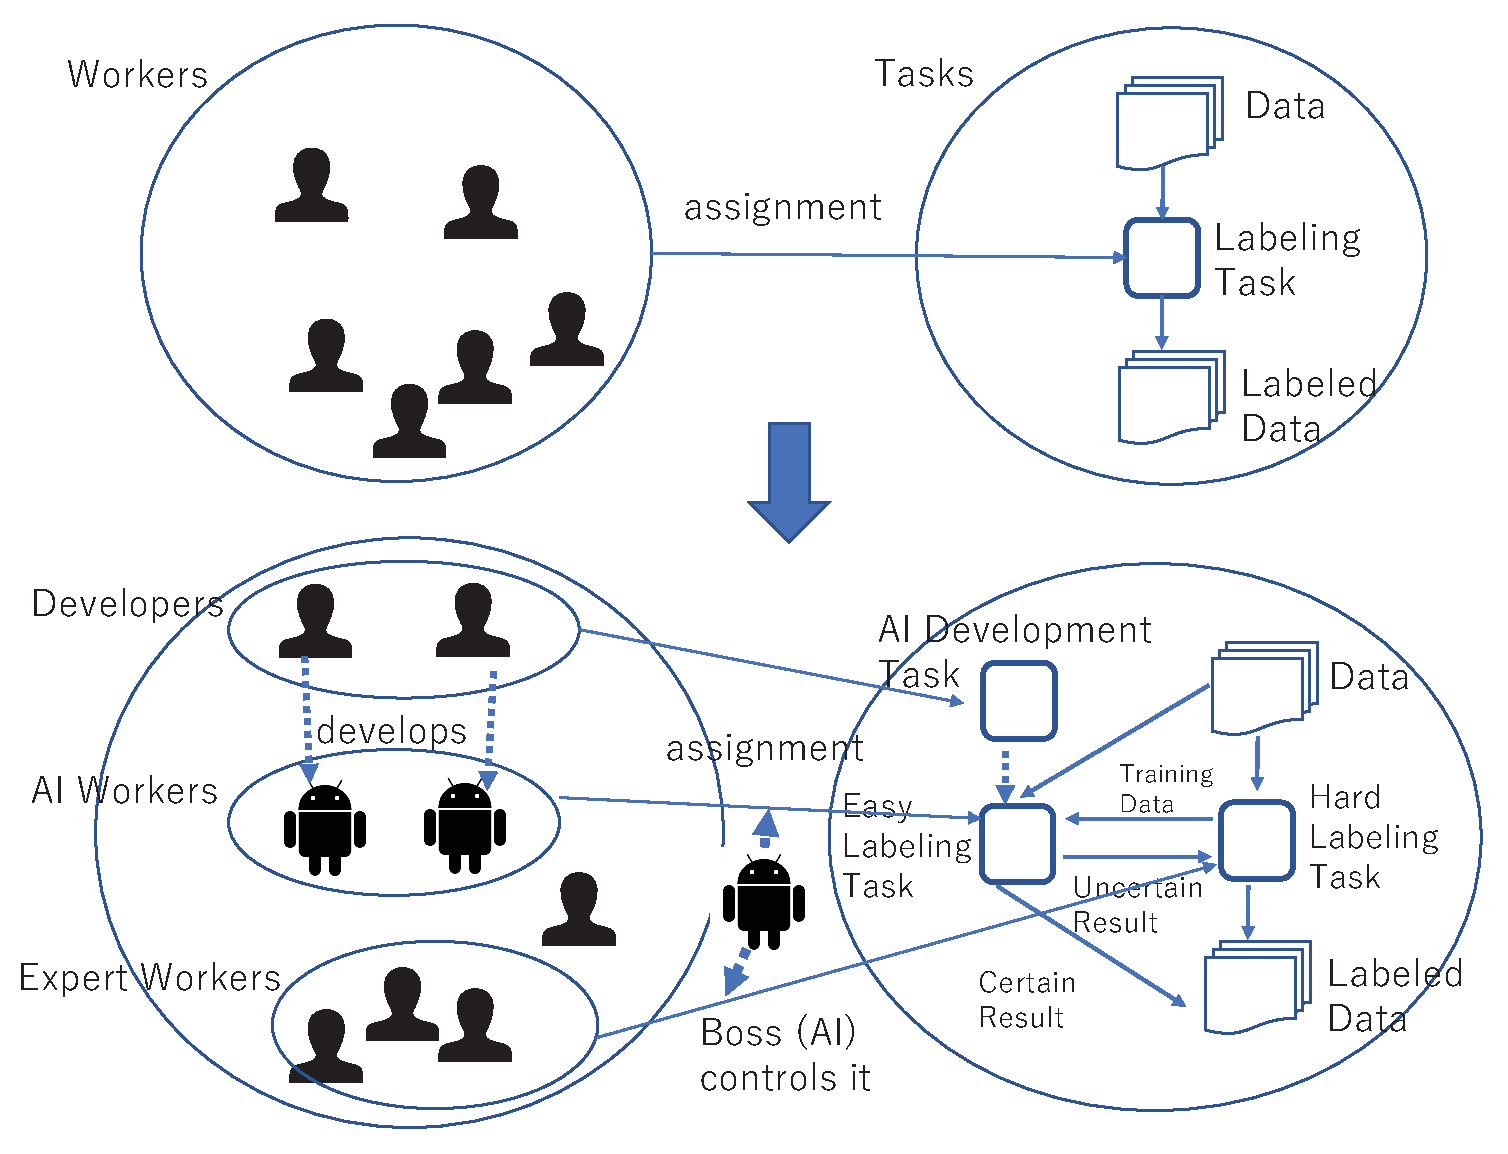
\includegraphics[width=100mm]{submissions_new/morishima/figures/dol-example1.eps}
    \caption{Example of dividing tasks and workers into multiple classes. If we know we have software developers in the worker pool, we can decompose the original task into a set of tasks consisting of AI development task, AI labeling task, and human labeling task. Since the tasks include tasks for AI workers, we recruit software developers so that AI workers are added to the worker pool.}
    \label{fig:example}
\end{figure}

The ``computational division of labor'' is not a new concept, and has been addressed in many related areas, notably in crowdsourcing research, although the state is still in its infancy as we will show in the next section.
%although the research in the these areas tend to focus on specific settings.

Figure \ref{fig:framework} shows the framework for computational division of labor.
It has two key components: {\it task classes} and {\it worker classes}. 
A task class defines a set of task instances that require a specific set of capabilities in order to perform them.
A worker class defines a set of workers having a specific set of capabilities.
The task and worker classes have {\it mutual dependence};
%, in that what are good task classes (e.g., task decomposition) depend on workers, and what are good worker classes (e.g., what capabilities are required) depends on tasks.
%It has two main components: workers and tasks, for which we have {\it mutual dependence} in the division of labor setting; 
i.e., good task decomposition results in
\[
\argmax_{T \in \mathcal{T}}\; \vec{f}(\mathcal{M}(W,T)),
\]
where $W$ is a set of workers, $\mathcal{T}$ is the collection of feasible task decompositions for $W$, $\mathcal{M}$ is the appropriate assignment from tasks to qualified workers, 
% $\argmax_T\; \vec{f}(\mathcal{M}(W,T))$ where $W$ is a set of workers, $T$ is a set of tasks, \mathcal{M} is the appropriate assignment from tasks to qualified workers, 
and $\vec{f}$ is the multi objective functions that define what is good assignment.
The functions may include a variety of things, including the result quality,  the expected cost due to mistakes, and human factors related to workers \cite{AR16}.
In the opposite direction, what skills workers should obtain and what kinds of AI workers should be developed are described by  
\[
\argmax_{W \in \mathcal{W}}\; \vec{f}(\mathcal{M}(W,T)),
\]
where $\mathcal{W}$ is the collection of sets of workers augmented by $T$, i.e., each $W \in \mathcal{W}$ can be a set of workers with new or better skills, or an extended set of workers with newly developed AI workers.
%$\argmax_{W}\; \vec{f}(\mathcal{M}(W,T))$, where $W$ can be the current set of  workers with new or better skills, or the workers extended with developed AI workers.
In addition, the set of skills the decomposed tasks require will affect 
how we should recruit workers.

Figure \ref{fig:example} gives an example process of computational division of labor for labeling tasks.
If we know that  we have software developers in the worker pool, we can decompose the original task into a set of tasks consisting of AI development tasks, easy labeling tasks (to be assigned to AI workers) and hard labeling tasks (assigned to human workers). Since the tasks include tasks for AI workers, we recruit software developers so that AI workers are added to the worker pool.

%depends on the required abilities $\{s| s\in requiredSkills(t), t\in T\}$ for completing decomposed tasks. 
%In addition, the  required skills and the number of tasks that require each skill will affect the learning and education policy for workers.
%The interaction between them are sometimes adjusted by ``invisible hands.''
Assignment of workers to tasks is often determined by  considering not only short-term benefits (such as time, quality, cost) for requesters, but long-term benefits, such as social sustainability and inclusion, with the three important benefits (skill improvement, low switching cost, and AI utilization) of division of labor considered.

The essential part of  division of labor in the framework is that there must be a variety of task classes, each of which requires different expertise or abilities to complete them.
Division of labor can lead to efficient society by exploiting the following advantages \cite{Smi76}:
%benefits:

\begin{description}
\item[Increase of Workers' Capabilities] Some tasks may require special expertise and workers need to have experiences or be trained for doing a good job on the task.
This sometimes requires long-term commitment of workers to a set of tasks that require particular capabilities.

\item[Lower Switching Cost] Cost for switching into completely new tasks  is generally high for humans. Taking into this factor when assigning tasks to human workers  increase the efficiency of manual labor. 

\item[Machine (AI) Taking Place of Manual Labor] Dividing the task into sub-tasks can increase the opportunities for machines (AI workers) to do the task, if the task is appropriately extracted so that the AI worker is capable of doing the task.
In order to achieve this, we need to address  meta-level algorithms that explicitly deal with capabilities of available AI workers.
\end{description}


\section{Related Research and Current Status}
\label{sec:relatedstatus}


%Although most of research generally focuses on the case where workers are human workers and the objective functions are given in terms of each workflow (e.g., quality, time, money), 
%it addresses many important issues in division of labor.
%However, computational division of labor is still in its infancy and there are many things researchers can do.

\eat{
Future-of-work is an area that focuses on worker's benefits in AI-driven job platforms, it addresses many human-centric issues for individual human workers. 
Computational division of labor is one of the ways to implement a better future of work.
}

There is a lot of research done related to computational division of labor. 
This section tries to organize relevant topics especially in the area of human-in-the-loop database systems, crowdsourcing and machine learning.
Although crowdsourcing research generally focuses on the case where workers are human workers and the objective functions are given in terms of each workflow (e.g., quality, time, money), 
there are papers that address important components of division of labor such as task and worker classes and the three benefits.
Human-in-the-loop database systems combine human and AI workers in the way that human workers collect data that are not stored in the current snapshot of database.
Regarding the division of labor between humans and AI workers, machine learning plays an essential role in some division of labor problems.
%Machine learners requires human workers to make training data in supervised learning.
Some studies such as supervised learning focus on addressing how to replace human labor by teaching AIs via a dynamic interaction between AIs and human workers.


\subsection{Dimensions and Overview}

Existing solutions for problems related to computational division of labor can be seen from the division of labor perspective by placing them in a space with the dimensions related to task and worker classes, such as follows:\\

\begin{figure}[t]
    \centering
    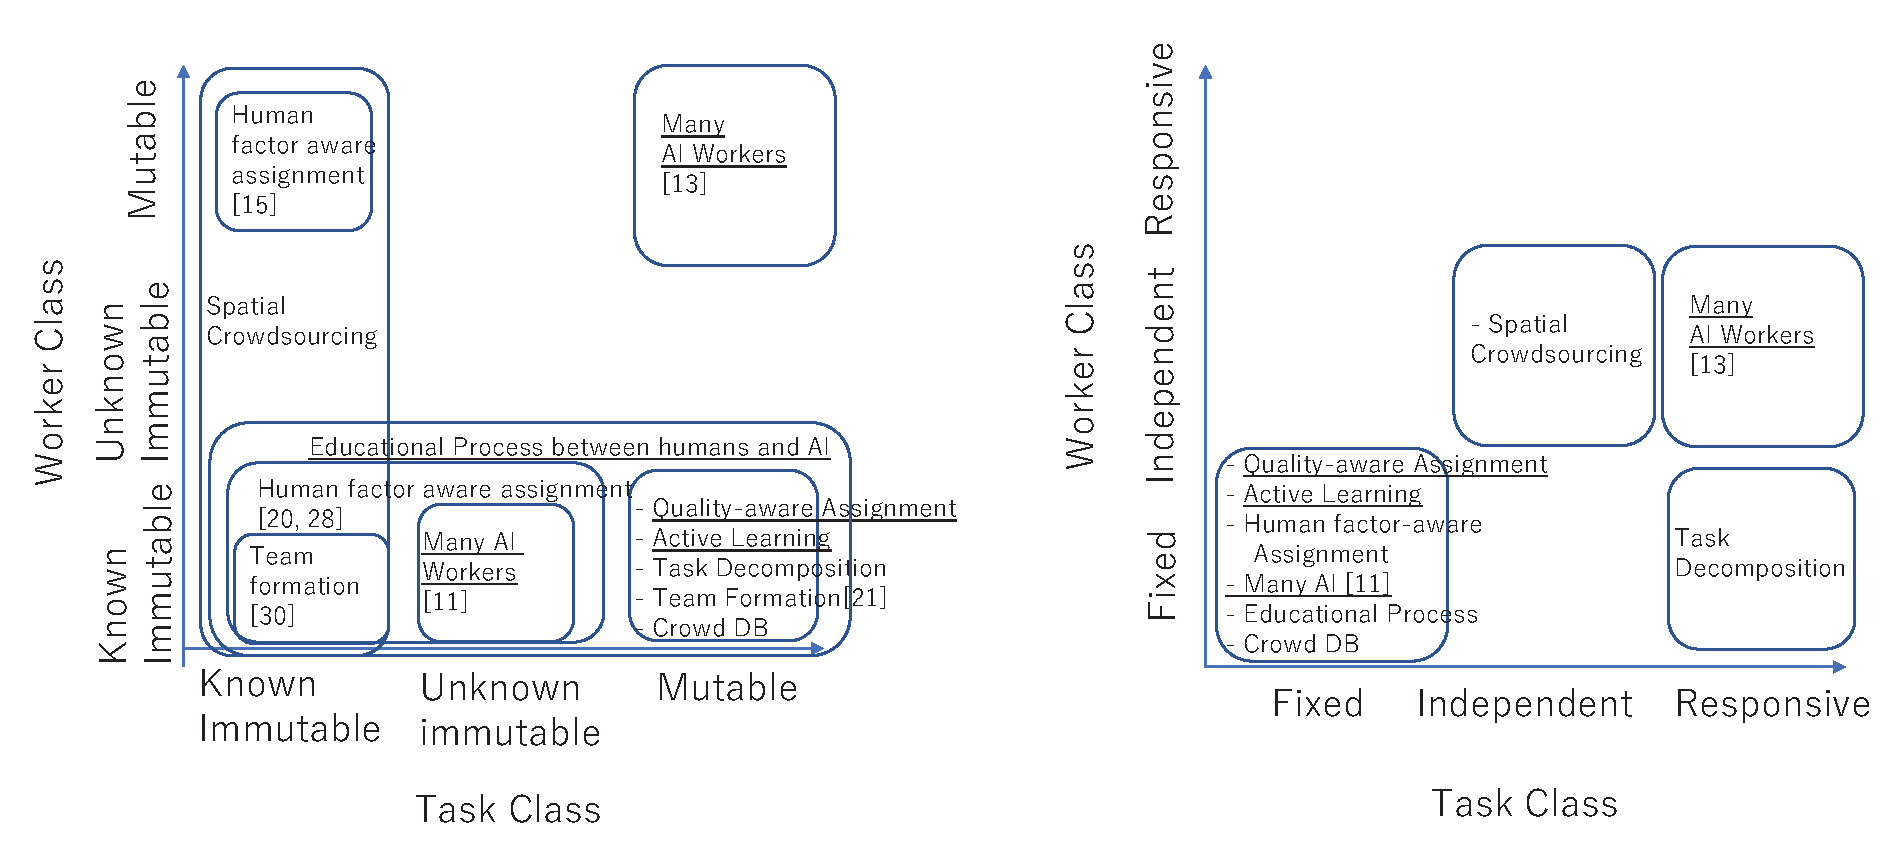
\includegraphics[width=160mm]{submissions_new/morishima/figures/dimensions.eps}
    \caption{Two views of a solution space of computational division of labor and the  current status of solutions in related topics. 
    On the left is the view with instnace-level mutability class dimentions.
    On the right is one with class-level dynamicity dimensions.
    Underlined Topics  deal with both of human and AI workers, while the others deal with human workers only.}
    \label{fig:dimensions}
\end{figure}

\begin{figure}[t]
    \centering
    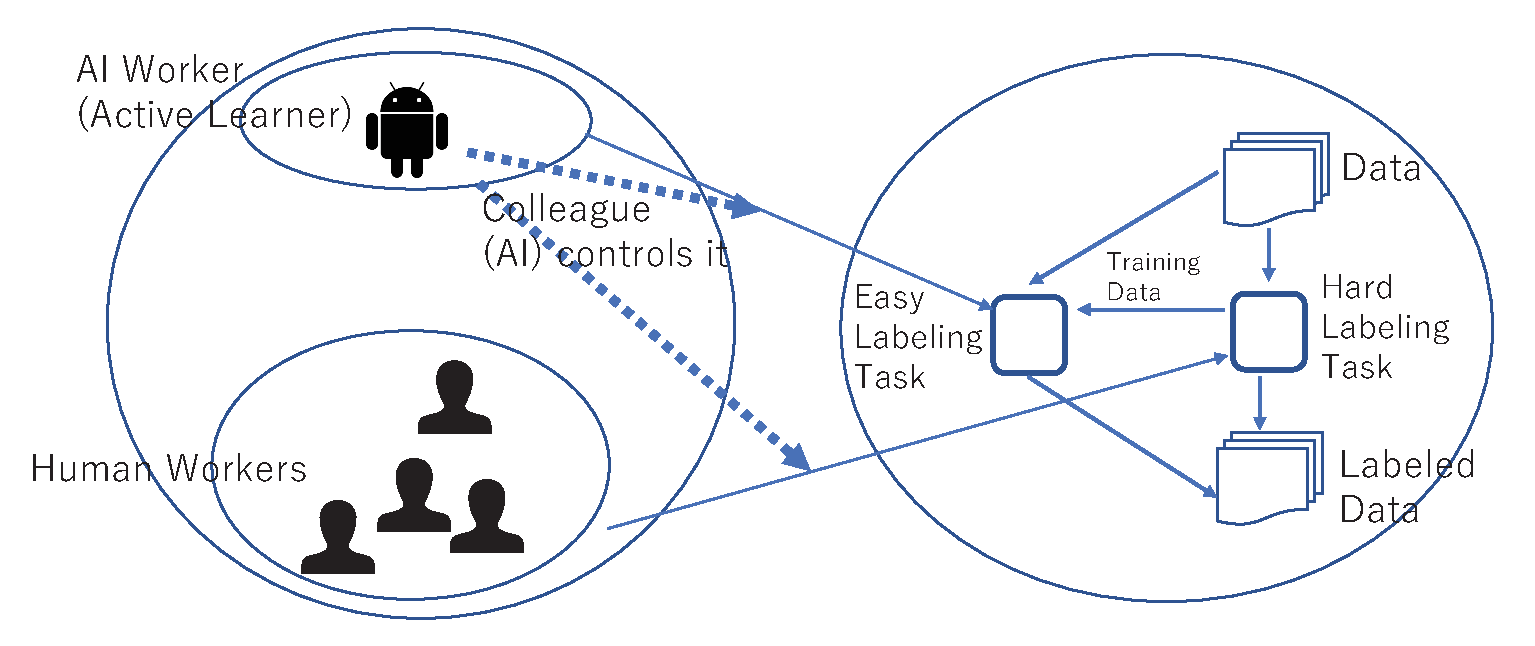
\includegraphics[width=100mm]{submissions_new/morishima/figures/dol-example2.eps}
    \caption{Active learning from the perspective of computational division of labor. The active learner is a colleague AI worker of human workers, who  controls the task assignment.}
    \label{fig:activelearning}
\end{figure}

\noindent
{\bf A. Instance level mutability of Task and Worker Classes.}
The dimentions represents the interaction between task (or worker) classes and their instances with  the three categories:

\begin{description}
\item[Known Immutable] The solution assumes that we already know which class each task or worker belongs to, and the instance-of relationship does not change.
\item[Unknown Immutable] The solution does not know which class each task or worker belongs to at first, but the instance-of relationship does not change once it decides the membership.
\item[Mutable] The solution changes the instance-of relationship according to a change of situation. Thus the number of instances of each class changes.
\end{description}

For example, some research papers classify crowd workers into novice and expert workers.
Other papers classify them into groups each of which contains similar workers in terms of accuracy per labels.
If a method assumes that we know who are  novice and expert workers in advance, it is labeled with ``Known Immutable.'' If a method measures the workers' skills and put them into classes only once, it is labeled with ``Unknown Immutable.'' If a method regularly checks the skills and changes the memberships accordingly, it is labeled with ``Mutable.''
An example with task classes is as follows: If a complex workflow is required in an application, the workflow may contain different kinds of tasks, such as find, fix  and  verification tasks  \cite{BLM+10}, which are connected to each other in the workflow.
If the solution takes as input such a workflow and does not decompose it, it is labeled with ``known Immutable.'' If a method decomposes the tasks into smaller ones, it is labeled with ``Mutable.''
Another example is the case where we have a set of data labeling tasks  and find a subset of the data labeling tasks  appropriate for training AI workers. Then the set of tasks will be a new task class. A method to find such a subset is either ``Unknown Immutable'' or ``Mutable'' depending on whether it updates it during the execution or not.\\

\eat{
This dimension represents two categories (fixed or dynamic) of worker classes each problem and solution in division of labor deal with. 
If worker classes can be added or deleted during the execution, the worker classes are dynamic. Otherwise, the worker classes are static.
For example, some research papers classify crowd workers into novice and expert workers.
Other papers classify them into groups each of which contains similar workers in terms of accuracy per labels.
Recently, AI agents are emerging as workers, therefore, how to involve AI workers is an important issue.
}

\noindent
{\bf B.  Class-level Dynamicity of Task and Worker Classes.}
The dimensions represent the interaction between task and worker classes with  the three categories:

\begin{description}
\item[Fixed] The solution assumes that the set of task or worker classes is fixed and always contains their instances.
\item[Independent] The solution allows that  task (or worker) classes can be added or deleted during the execution, and such operation is done independent of  worker (or task) classes.

\item[Responsive] The solution adds or deletes tasks or worker classes during the execution, and the action is affected by the situation in their counterpart (e.g., changes in worker classes cause the division of task classes). 

\end{description}

For example, a task decomposition method may not look at available workers  at all. Such a method is labeled with ``Independent.'' Another may consider the current availability of workers before the task decomposition. Such a method is labeled with ``Responsive.''
Responsiveness is definitely the potential benefit of computational division of labor, which will be useful in situations such as COVID-19 pandemic where we encounter a sudden change in labor resources.
%(offline to online, for example).

\eat{
\item[Task Classes]
This dimension represents two categories (fixed or dynamic) of task classes each problem and solution deal with. 
If task classes can be added or deleted during the execution, the task classes are dynamic. Otherwise, the task classes are static.
If a complex workflow is required, the workflow may contain a different kinds of tasks, such as fix  and  verification tasks, which are connected to each other in the workflow \cite{BLM+10}.
This way, the output of a task sometimes is the input of another task.
Another case where we have multiple task classes is when we have subclasses of a particular task class. Subclasses can be defined with its contents or attributes (such as locations for spatial tasks).
%A task class may be divided into more than one subclass. For example, classification tasks may be organized in a hierarchical structure where upstream tasks classify data items into rough categories and each of  downstream tasks give labels in each category.

\item[Responsiveness]
This dimension represents to what degree the relationships between workers and tasks (i.e., education, recruitment, assignment, and decomposition) are responsive to the condition change. 
In other words, how often the status of workers and tasks affects each other. For example, a task decomposition method may not consider any attributes of available workers (not responsive at all), another may consider them once before the task decomposition, or a more responsive approach may periodically look at changes of the status of worker pool and updates the task decomposition accordingly.
Responsiveness is definitely the potential benefit of computational division of labor, which will be useful in situations such as COVID-19 pandemic where we encounter a sudden change in labor resources (offline to online, for example).
}

\eat{
\item[Assignment Flexibility]
This dimensions represents to what degree the assignment is constrained by the classes of workers and tasks. 
In other words, it represents whether the many-to-many  mapping (assignment) between classes of workers and tasks are allowed or not. The assignment will be more flexible if the workers move among worker classes when their attributes change (e.g., skill improvement) when the workflow takes a long time to complete.
}
%\end{description}

Figure \ref{fig:dimensions} puts some of the related topics (details will be shown in Figure \ref{fig:relatedwork}) in the three dimension space. 
The results show that, at this moment, there are a limited number of studies that deal with  responsive class generation. They deal with the two cases where (1) they assume human workers only and do not deal with automatic task decomposition and workflow optimization, and (2) they deal with human and AI workers for simple data labeling tasks. In contrast, there are few studies that deal with dynamic task and worker classes containing AI workers. Many studies focus on dynamicity of either worker or  task classes only.
Among the three benefits of division of labor, few studies focus on the problem of lowering switching cost. Some address the problem of improving workers' skills, and having Machine (AI) take place of manual labor, but the they addressed the problems independently.
Most of the objective functions are defined in terms of short-term, requester-centric views on each workflow.\\
 %There are only a limited cases to deal with 
 %However, in many cases, we have limited responsiveness. For example, task decomposition and quality-aware assignment considers the status of worker pool once, or even if responsive, the change is manual.


\noindent
{\bf C. Controller of Division of Labor.}
In addition, there are different approaches on who controls the division of labor. 
The followings are potential subjects that  control the division of labor process.
\begin{description}
\item[Boss] There are approaches that assume a subject other than workers, who mainly takes care of the task decomposition, assignment, recruitment, etc. The boss can be a human, an AI agent, or a human-in-the-loop algorithm.
\item[Colleague] There are some cases where one of the workers decides who perform what tasks.
For example, we can view active learning methods in the division of labor perspective as follows. We have two types of workers (a machine learner and humans), where the decision maker who assigns tasks for data labeling is the learner (Figure \ref{fig:activelearning}).
\item[No one] There is nobody who explicitly controls  the division of labor. Rather, how it goes is incorporated in the design of the framework, such as incentive design, to implement ``invisible hands.'' 
The task decomposition, assignment, education, recruitment, etc. are implemented as the result of every participant's action in the process of pursuit of their own gain.
\end{description}







%In the division of labor context, the development of AI and the online infrastructure allows us to not only do computationald division of labor, 



\eat{
\begin{itemize}
    \item Online Job platforms such as crowdsourcing services, share rides,  Computational Division of labor is an optimization of The trend of Future-of-Work, 
    \item In the near future, the workforce Online jobs are 分業は重要
    \item In the near future, all tasks will be human in the loop
\end{itemize}
}



\eat{ // old version
\begin{figure}[t]
   \scriptsize
    \centering
\begin{tabular}{|p{19mm}|p{10mm}|p{22mm}|p{18mm}|p{29mm}|p{30mm}|p{15mm}|}
\hline
Topic&Examples&Task
Classes&Worker Classes&Responsiveness&Objective Functions&Controller\\
\hline
\hline
Quality-Aware Microtask Assignment & \cite{NWL15}&One &Three (Novice, Expert, AI)& Automatic assignment, but no worker movement among classes& Better quality with a limited budget&Boss (AI)\\
\hline
Spatial Crowdsoucring Task Assignment    &\cite{TZZ+20} &One (human workers), but there are many sub-classes for different locations& One, but divided into many subclasses by their locations& Automatic many to many assignment, considering the distance between locations of tasks and workers& Maximizing total number of assignments,Optimized for average performance, Maximizing total payoff, etc. &Boss (AI)\\
\hline
Active Learning   &\cite{YRF+11,RPR14,ZC15,HHM+15} &One (data labeling)&Two (AI and Human)&Dynamic assignment of tasks based on estimation of worker's skills&Better machine learning models& Colleague (AI) \\
\hline
Working with a Large Number of Data Labeling AI Workers& \cite{KWM20} &One (data labeling)&Two (AI and Human)&Automatic task assignment based on dynamic estimation of AI performance&Quality and speed of task completion&Boss (AI)\\
\cline{2-7}
& \cite{KWM20b} &One (data labeling)&Two (AI and Human)&Task prioritization once before assignment&Better performance of AI Workers&Boss (AI)\\
\hline
Task Decomposition&\cite{KCH12} &Many&One (human workers)&Assumes every task always have enough workers&Each task must be done for a fixed price&Boss (human workers)\\
\hline
Team Formation &
\cite{VRT+17}
&Complex works e.g. product design, software development, and game production.
& Many (All human).
& Automatically hire expert crowd workers into roles and  manually reconfigure the role structure during the execution.
&Organizing the teams to accomplish complex work.
& Colleague (Human) and requester\\
\cline{2-7}
&\cite{RRT+19}&Many&Many&Optimally form groups with available workers pool&Affinity and upper critical mass with skill and cost constraint&Boss (AI)\\
\hline
Human-Factor Aware Microtask Assignment&
\cite{KMS+18}&One (speech transcription)&Many (different skill levels)&Iterative and automatic task assignment to groups&Skill, Psychological Stress&Boss (AI)\\
\cline{2-7}
&\cite{SBB+14}&One (Image classification)& Many (different skill levels) & Iterative update of workers state& Learning &Colleague (AI)\\
%\cline{2-6}
%&\cite{YHX+18}& &&& skill & Boss (AI)\\
\cline{2-7}
&\cite{PAS+18}&Many&Many (different human factors)&Iterative task assignment&Worker Motivation, Task relevance & Boss (AI)\\

%\hline Human-AI task assignment& \cite{KWM20} &One&Two (machine and Human)&Yes&Obtain the results with the quality guarantee\\
%\hline
%Complex Crowdsourcing &Deco&&&&\\
%\cline{2-6}
%&&&&&\\
\hline
Educational Process between Human and AI & \cite{YXG18,LDH+17,FZL+12,JAB15} & One (data labeling) & Two (AI and human) & AI learns effective teaching schemes and humans get higher ability to the task. & Educating machines and humans to obtain better results. & Colleague (AI)\\
\hline
Crowd Databases &\cite{FKK+11, PPG+12}& Many (filtering, join, etc.) & Two (Humans and DBMS) & Workflow optimization is static and based on the data statistics& Monetary cost, Time, Quality&Colleague (AI)\\
\hline
\end{tabular}
    \caption{Division-of-Labor view of some of  related  research topics that deal with at least more than one worker  or task class or address important benefits in division of labor}
    \label{fig:relatedwork}
\end{figure}
}

\begin{figure}
   \scriptsize
    \centering
\begin{tabular}{|p{15mm}|p{10mm}|p{24mm}|p{24mm}|p{35mm}|p{24mm}|p{13mm}|}
\hline
Topic&Examples&Task Classes and Relationship with their Instances&Worker Classes and Relationship with their Instances &Class-level Dynamicity and Interaction&Objective Functions and Constraints&Controller\\
\hline
\hline
Quality-Aware Microtask Assignment & \cite{NWL15}& Three subclasses (Crowd, Expert, AI) of a data labeling task class. Mutable %(the same task will be categorized into other classes later)
&Three classes (Crowd, Expert, AI). Known Immutable %(Workers do not move among classes)
& No change at task and worker class levels.
%Fixed set of task and worker classes, each of which assumes to have instances in it. 
& Better quality with a limited budget&Boss (AI)
\\
\hline
Spatial Crowdsoucring Task Assignment    &\cite{TZZ+20} &Subclasses of a spatial task class  with different locations. Known Immutable& Classes for human workers in different locations. Known Immutable or Mutable& Task and Worker classes  can be added and deleted dynamically, but independent of each other.
& Maximizing total number of assignments, Optimized for average performance, Maximizing total payoff, etc. &Boss (AI)\\
\hline
Active Learning   &\cite{YRF+11,RPR14,ZC15,HHM+15} &Subclasses (easy and hard) of a data labeling task. 
%Some methods have sub-classes of the hard task class. 
Mutable&Two classes (AI and Human) known Immutable.
%Some methods have sub-classes of the human worker classe with different skill levels
&
No change at task and worker class levels.
% Some assumes dynamic task classes with different difficulties or worker classes  with  different skills.
%[Task and worker classes are fixed] Assignment of tasks based on estimation of worker's skills
&Better machine learning models& Colleague (AI) \\
\hline
Working with a Large Number of Data Labeling AI Workers& \cite{KWM20} &Subclasses of a data labeling task class for human and AI workers. Mutable %(tasks are re-assigned)  
& One human worker class and many AI worker classes for different skills. Unknown Immutable&  Automatic subclass generation and assignment triggered by dynamic estimation of AI worker performance&Quality and speed of task completion&Boss (AI)\\
\cline{2-7}
& \cite{KWM20b} &Two classes for easy and hard labeling tasks. Unknown Immutable. &Two classes for AI and Human. Known Immutable &Task classes are computed once based on a task prioritization algorithm before assignment&Better performance of AI Workers&Boss (AI)\\
\hline
Task Decomposition&\cite{KCH12} &Many dynamically-generated classes. Mutable.  &One (human workers). Known immutable. &Task classes are dynamically generated,
according to workers' judgement.
%assuming  that every task class are assigned to the only one worker class
%Assumes every task al-ways have enough work-ers
&Completing tasks with the crowd. Each task must be done for a fixed price&Boss (human workers)\\
\hline
Team Formation &
\cite{VRT+17}
& Many classes with different roles. Anyone can propose new role and edit role structure.
Mutable.
& Two (Team leader and team members). Known Immutable
%All team members are hired from crowdsourcing platform. Immutable?.
& Task classes are first defined by the leader, but can be reconfigured manually by anyone during the execution.
%expert crowd workers into roles and  manually reconfigure the role structure during the execution.
&Organizing the teams to accomplish complex work with deadline of six weeks and budget.
& Colleague (Human) and Boss (Human)\\
\cline{2-7}
&\cite{RRT+19}&Complex workflow consists of several tasks that require different capabilities.
Known Immutable &
Many classes with different capabilities and wage expectation. Known Immutable &
No change at task and worker class levels. The algorithm optimally forms groups with available workers pool &
Worker-worker affinity and upper critical mass with skill and cost constraint&Boss (AI)\\
\hline
Human-Factor Aware Microtask Assignment&
\cite{KMS+18}&One for speech transcription. Known Immutable & $N$ subclasses. Workers are divided into each subclass based on current skill distribution.
Mutable & No change at task and worker class levels. &Skill, Psychological Stress&Boss (AI)\\
\cline{2-7}
& \cite{SSL+16}&Each task will be broken down by the mentor into several subtasks only once. Unknown Immutable.
& Two (Mentor and Intern worker). Known Immutable.
& No change at task and worker class level.
& Better learning of intern worker
& Boss (Human)\\
% &\cite{SBB+14}&One for image classification. Known Immutable & Many with different skill levels. Unknown \& mutable & 
% No change at task and worker class level.
%Iterative update of workers state (問合せ中)
%\cline{2-6}
%&\cite{YHX+18}& &&& skill & Boss (AI)\\
\cline{2-7}
&\cite{PAS+18}&Many: each task has different content and requirements associated to keywords. Known Immutable & Many: each worker has different interests associated to keywords. 
Known Immutable &
No change at task and worker class level.
However, correspondences between task and worker classes are dynamically changed.
&Worker Motivation, Task relevance, and Task diversity& Boss (AI)\\

%\hline Human-AI task assignment& \cite{KWM20} &One&Two (machine and Human)&Yes&Obtain the results with the quality guarantee\\
%\hline
%Complex Crowdsourcing &Deco&&&&\\
%\cline{2-6}
%&&&&&\\
\hline
Educational Process between Human and AI & \cite{YXG18,LDH+17,FZL+12,JAB15} & Two classes (tasks for education and not) of data labeling tasks. They are Known Immutable in \cite{JAB15}, and Mutable in the others. & Two classes (Human and teaching AI). 
Known Immutable. & No change at task and worker class level. & AI learns effective teaching schemes and humans get higher ability to the task. & Colleague (AI)\\
\hline
Crowd Databases &\cite{FKK+11, PPG+12}& Many Tasks (filtering, join, etc.). Mutable & Two (Humans and DBMS). Known Immutable & Task classes are determined in the optimization phase based on the data statistics and fixed before the execution.
& Monetary cost,  
Quality&Colleague (AI)\\
\hline
\end{tabular}
    \caption{Division-of-Labor view of some of  related  research topics that deal with at least more than one worker  or task class or address issues related to benefits of division of labor}
    \label{fig:relatedwork}
\end{figure}


\subsection{Computational Division of labor View of Existing Studies}

Figure \ref{fig:relatedwork} shows some of the related works that satisfy one of the following conditions: (1) The work deals with more than one task or worker classes (2) the work addresses issues related to benefits of division of labor - increasing workers' capabilities, lower switching cost, and AI workers taking place of manual labor.

\noindent
{\bf Quality-Aware Microtask Assignment.}
For finite pool data categorization, there are approaches to assign appropriate tasks to different classes of workers to  improve the result quality. 
For example, \cite{NWL15} discusses how to assign the categorization tasks to  two categories of human workers, namely, experts and crowd workers, and an AI worker (a classifier model), in order to achieve high quality results. 
In the method, the AI worker is considered as a worker that responds to all the tasks that have been assigned to no human workers when the budget is run out.
The method dynamically estimates the result quality in a situation that we train the AI worker with tasks labeled by humans and assign the rest of tasks to the trained AI worker.
In terms of class-level dynamicity, it does not change task or worker classes during the execution. Furthermore, it always assumes to use a particular AI worker whose algorithm is known and does not accept AI workers that are developed by crowd workers.

%若林先生,[NWL15]はここで良いでしょうか?良いかもですが. => たぶん良い


\noindent
{\bf Spatial Crowdsourcing.}
In spatial crowdsourcing, tasks and workers are associated to locations. 
Logically, we can think of many subclasses of each of the task and worker class, defined by their locations.
The (sub-)class of each task or worker is known because we know their locations. 
In some settings, workers move thus the the worker classes they belong to are mutable.
The task (worker) classes can be added and deleted dynamically as their instances appear and disappear, independently of workers (tasks).
%The task assignment is flexible in that potential workers for a task are in more than one worker class and the assignment is automatically computed.

\eat{
deals with many worker and task classes, which are subclasses of  one worker and task class, respectively, by the locations of workers and tasks. Although the assignment is flexible in that potential workers for a task are in more than one worker class, the worker (sub-)classes exist regardless of task classes and vice versa. 
Although there are many subclasses defined by locations, they all are subclasses of the only one task that require the same skill set of workers.
}

\noindent
{\bf Active Learning.}
Active learning interacts with human workers to (i) ask humans to make training data for data instances specified by {\it an AI worker} and (ii) receive the training data from humans to better learn the way to work \cite{Set09}.
Some active learning methods are aware of the performance of each worker and assign tasks to specific workers \cite{RPR14,YRF+11}.
In this discussion, we need to clearly distinguish the two roles of AI workers;  a controller of task allocation to task classes and a task executor.
The task allocation controller is a subject that organizes the dynamic allocation of data labeling tasks to the task class for human workers (i.e., hard task class), while a task executor is a subject that accomplishes data labeling tasks that could be assigned to human workers.
From the viewpoint of the division of labor between humans and AIs, it is helpful to recognize that these active learning systems play two different roles because we potentially can find more flexible way to design AI components, e.g., working with a large number of task executor AIs, which we explain later.
While the typical goal of active learning is to take over the human labor on data labeling tasks as a task executor, the allocation function is elaborated in some active learning models proposed so far.
For example, Fang et al. \cite{FZL+12} proposed an active learning model that encourages human learning by selecting a pair of workers having different skills to work together on the same data labeling task.
Another example can be found in active learning that dynamically estimates the difficulty of tasks and assign only difficult tasks to workers of domain expert for minimizing the labor cost \cite{HHM+15,NWL15,ZC15}.
In terms of class-level dynamicity, no change happens on the task an dworker classes in  active learning systems.

%\cite{KWM20}.

\begin{figure}
    \centering
    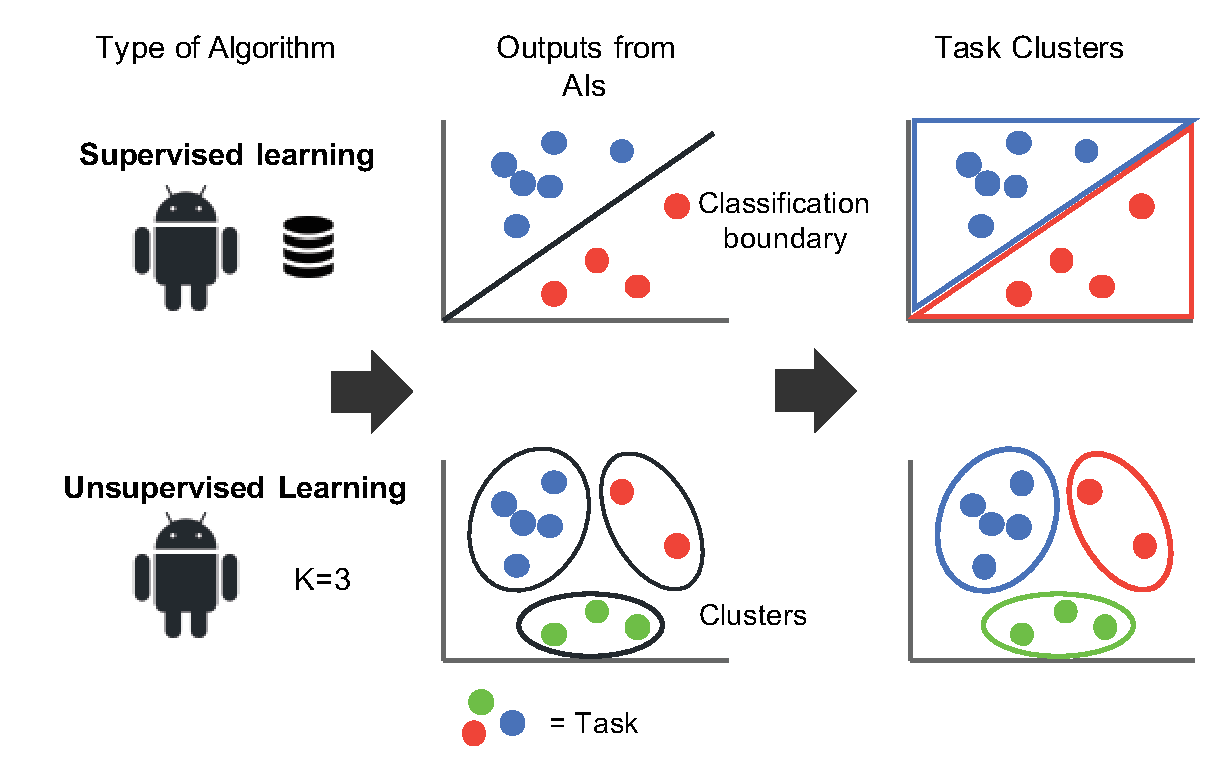
\includegraphics[width=70mm]{submissions_new/morishima/figures/task_cluster.eps}
    \hspace{10mm}
    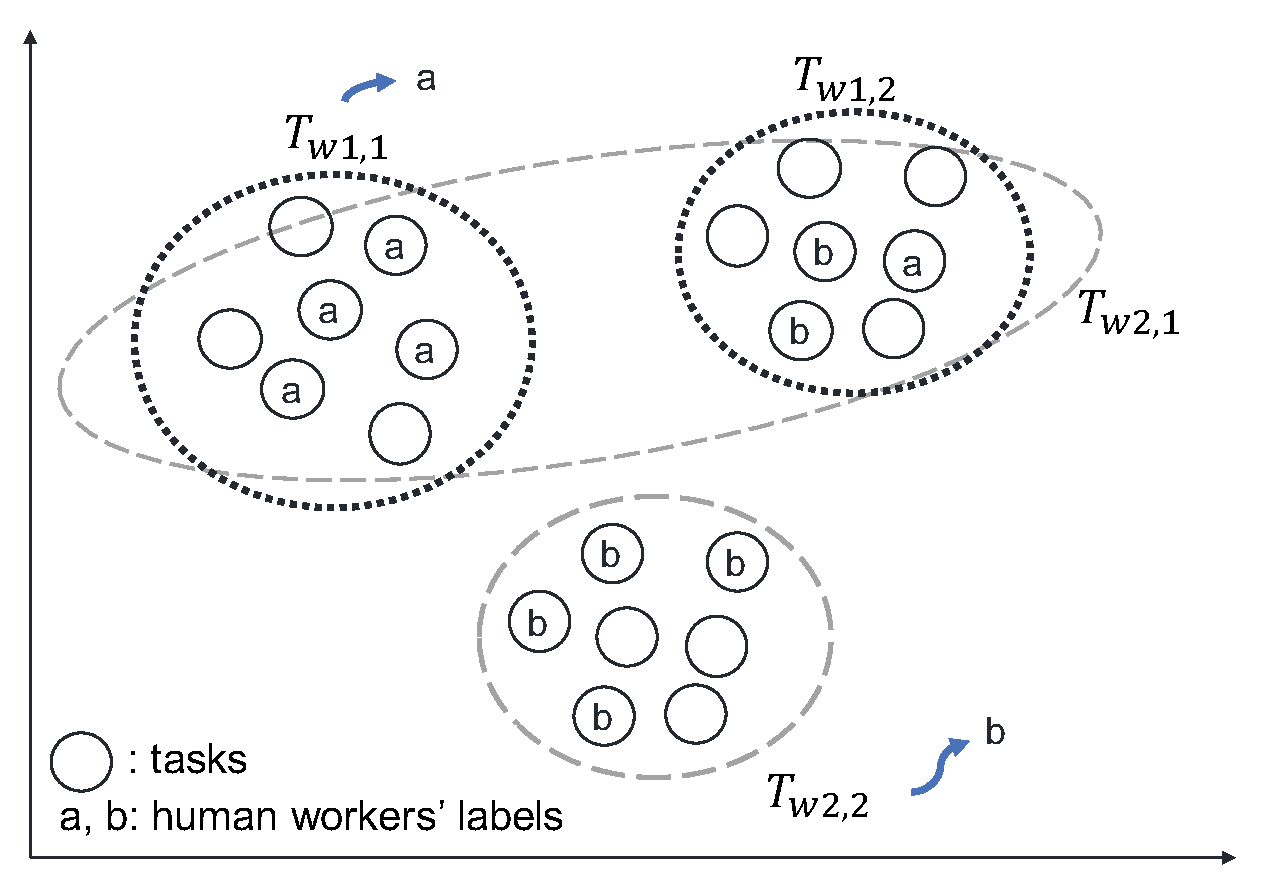
\includegraphics[width=70mm]{submissions_new/morishima/figures/proposed_method.eps}
    \caption{The method proposed in \cite{KWM20}. Each AI worker is assumed to cluster tasks, regardless of how it is implemented (left). The method conducts statistical tests to find whether all tasks in each task cluster is associated to a particular label, by looking at the labels given by human workers (Right). Here, $T_{w_{i,j}}$ means the $j$th task cluster of AI worker $i$. {\tt a} and {\tt b} are labels given by human workers.}
    \label{fig:hactap}
\end{figure}

\noindent
{\bf Working with a Large Number of Data Labeling AI Workers.}
There are studies on labeling a finite number of data items with not only human workers but also {\it a large number of} AI workers.
The paper \cite{KWM20} proposes HACTAP  (Human+AI Crowd Task Assignment Problem) that allows black box AI workers to join the workflow during its execution and assigns tasks to them if the high quality result is expected.
Figure \ref{fig:hactap} shows the proposed method shown in \cite{KWM20}.
Their method does not assume any particular model implemented in each AI worker. Rather, they assume that each AI worker outputs task clusters (which correspond to task (sub) classes in this paper) (Figure \ref{fig:hactap}(left)).
A task cluster will be meaningful if all tasks in each task cluster are associated to the same label.  Therefore, the method conducts  statistical tests to know whether each cluster corresponds to a particular label, by looking at the labels given by human workers. If the task cluster passes the test, all tasks in the cluster will be assigned to the AI worker.
The method allows dynamic task assignment according to the available AI workers at each time, but the workflow is limited to a simple labeling task. 
The paper \cite{KWM20b} presents a batch prioritization of data labeling tasks that allows a large number of black box AI workers to be efficiently trained. 
It statically assigns tasks to humans in advance before the task execution so that it effectively train AI workers independent of their underlying models. Thus, it can train a large number of blackbox AI workers with different underlying models in parallel. 
In terms of class-level dynamicity, there are only two fixed classes for tasks and workers. However, their hard labeling tasks are carefully chosen so that the tasks are effective for training AI workers with any underlying models.

\noindent
{\bf Task Decomposition.}
There are studies to ask human workers to do task decomposition.
For example, \cite{KCH12} proposes the PDS (Price-Divide-Solve) algorithm to ask crowd workers to decomposed tasks into smaller ones. The result workflow contains a diverse set of microtasks whose results are merged to produce the final product. Worker classes are not explicitly dealt with in the algorithm, but they assume that each task is done with the fixed payment (20 cents, in their implementation). This implies that it assumes that the task is easy enough so that we can easily find workers that do the task with the payment in crowdsourcing platforms.

\noindent
{\bf Team Formation.}
There are studies on how to configure teams to solve complex problems.
\cite{VRT+17} proposed flash-organization which enables us to hire expert crowd workers into role structures and dynamically reconfigure the structure via version control.
\cite{RRT+19} proposed an optimization model for task assignment in a collaborative crowdsourcing environment and proposed optimization algorithms with theoretical guarantees.
From the aspect of the computational division of labor, \cite{VRT+17} allows  human workers to change task classes, but it is not automatic, while \cite{RRT+19} performs automatic task assignment at class-level, but does not allow dynamic change at the class level. Assignment to AI workers is not discussed in both of them.

\noindent
{\bf Human-Factor Aware Microtask Assignment.}
While many crowdsourcing studies have assumed that anonymous workers have the same role, every human being is different, i.e. what tasks the workers are good at, what motivates them, and what they are doing the task for, are different for each person.
%For this reason, the studies often focus on task assignment from the requester's perspective. 
Thus, considering the human rights of workers, it is natural to take into account the worker's perspective, in other words, it is important to consider who, when, and which task should be performed by whom. Therefore, the number of worker class is usually plural in this topic.
Recently, the importance of human-factor in crowdsourcing has been argued \cite{AR16}, and task assignment research has been addressed in line with this perspective. For example, \cite{KMM+18} considers psychological stress, \cite{PAS+18} considers motivation, and \cite{SSL+16} considers worker's learning.
Class-level dynamicity is not addressed in this topic.

\noindent
{\bf Educational Process between Humans and AI.}
Assigning a task to workers with appropriate ability is important for efficient problem solving.
Increasing workers' skills is an important issue in division of labor,  from the viewpoint of obtaining high-quality task results in the long term.
%, it is important to develop the skills of workers.
%Assigning a problem to workers with appropriate ability is important for efficient problem solving, however, from the viewpoint of obtaining high-quality task results in the long term, it is also important to develop the skills of workers.
For this problem, there are studies dealing with the interactive educational process between humans and AI.
In this process, the AI learns the optimal task assignment to maximize the learning effect for human workers.
These researches give us new insight into the task division from the viewpoint of the cultivation of expert human workers.
However, the existing studies discuss improving skills {\it within} a particulars task class. 
From the division of labor view, it is important to address the problem of  improving skills across task classes in different workflows.  

\noindent
{\bf Crowd Databases.}
Crowd Databases such as CrowdDB\cite{FKK+11} and Deco\cite{PPG+12} employ human workers to obtain data that are not stored in the current snapshot of database in the  storage.
The workflow contains a variety of tasks such as data entry, selections, join, ordering, while it does not explicitly deal with worker classes and attributes. The optimization of workflow is based on the data statistics, rather than worker availability and their skills. 

\eat{
\begin{itemize}
    \item Automatic Tuning
    \item Schema Matching
\end{itemize}
}




%assuming a particular set of workers, ways (crowdsourcing), nor topics, but shows a set of criterion on what are good task decomposition and assgnment. and computational division of labor is an approach to use computations for good task decompositions and assignment in the division of labor aspect.
%People have been addressing part of computational division of labor problems, in many reasearch area, such as crowdsourcing. 
%This paper uses the term computational division of labor, because the problems have been dealet with in many research topics.
%problemsrelated not to a parmany research areas.
%many other terms stress that they address problems in a particular context, but 

\eat{
Topics in division of labor problems spans from low-level problems such as assignemnt of a set of given tasks to a specific set of workers, to high-level problems such as $\ldots$. %a 
holistic view. The following explains what computational division of labor is and isn't.
\begin{itemize}
    \item Division of Labor often deals with problems at the society level. For example,  how to implement ``invisible hand'' is an important issue in computational labor.
    \item Division of labor does not require the task to be done by the crowd. The task may be completely addressed by AI agents, if it is appropriate. This is a contrast to crowdsourcing research.
    \item Role assignment is an important issue in Division of Labor. For example, many existing researches address the problems on collaboration between AI and humans (such as Active Leaning), but each of such a research assumes a particular role assignment. Division of Labor requires us to address which role assignment is better, for integrating or switching many assignment techniques.
    \item Computational division of labor gives a means to implement an aspect of a better ``Future of Work'', in terms 
    
    \eat{    of they assume that they are  deals with a division of labor problems, in that it decides which tasks should be assigned to humans and learner, but if whDivision of labor o
    the the principles for task assignments, to advance the wealth of human beings.
    \item Crowdsourcing is a way to achieve a particular goals by recruiting people from the crowd and to ask them to perform their tasks.
    \item Future of Work focuses on the worker's issues in the advanced work environments.
    }
\end{itemize}
}

\eat{
\begin{figure}
    \centering
    \begin{tabular}{|l|l|}
    Category&Research Issues\\
    Skill Improvement& Skill Improvement, Skill-aware task assignment\\
    Low switching cost& Switching-cost aware Task Assignment (e.g., batch)\\
    Adoption of Machines& Working with AI, Task Assignment to AI algorithms and machines
    \end{tabular}
    \caption{Classification of existing research in terms of computational division of labor}
    \label{fig:fig-x}
\end{figure}
}

%\subsection{Division of Labor in Data Engineering and Management}

% 8/24 ひとまず入れて見ました(鈴木)
% 8/28 4.1は隠し,4.2をopen problemsへ移すことにする
%\section{Formal Aspects of Computational Division of Labor}

\subsection{Computational Model and Complexity}
 
As with conventional computation in computer science, computation in
computational division of labor also takes some input, does some
computation along with some algorithm, then outputs some
result. However, now AI or human workers participate in computation,
which affects the way of computation itself. Therefore, (a)
establishing a formal computation model covering such factors and (b)
investigating computational complexity under such a model are of great
interest. As a preceding study, a computation model for crowd data
mining is proposed and computational complexity of several problems on
the model is investigated \cite{AM14}.

Here, let us consider a more general case in which we have a workflow
$W$ with tasks $t_1,t_2,\cdots,t_n$. In this case, task $t_i$ is
``computed'' in {\em one step\/} by an AI/human worker. Here, suppose
that the complexity of task $t_i$ is in class $C_i$ (PTIME, NP,
etc.). Then the computation of $W$ would be modeled as a Turing
machine with a set of oracle $C = \{C_1,C_2,\cdots,C_n\}$. But this is
still too simplified, off course, and we have a number of things to be
considered.
\begin{itemize}
\item How the computational power of workers affects workflow is an
  essential problem of computational division of labor. What makes
  workers, especially human workers, different from machines is that
  workers sometimes report incorrect answers but can respond to
  ``hard'' problems instantly with intuition. If we can estimate
  worker's computational power in any way (this is also an interesting
  problem), workflow using workers can be modeled as oracle machine,
  and we may be able to discuss computational power of such
  machine. For example, suppose that each worker has enough
  computational power to solve problems in PP, i.e., solve such
  problems in polynomial time with an error probability of less than
  $1/2$, and that workflow $W$ (without oracle) covers class P. Then
  the computational power of $W$ with oracle covers class
  ${\rm P}^{\rm PP}$. Note that
  ${\rm PH} \subseteq {\rm P}^{\rm PP}$~\cite{Tod91}, which would
  imply that $W$ can solve PH problems in polynomial time! Although
  this may be an extreme case, investigating how the computational
  power of workers affects workflow would be of great interest.
   
\item In conventional computation, algorithm is usually ``static'';
  different input values are given at each time but the algorithm
  itself is {\em fixed}. However, in the context of computational
  division of labor, workers and tasks affect each other, and both
  workers and tasks changes dynamically. In other words, workflow and
  tasks ``evolve'' over time along with changes of workers. Such
  dynamic aspects of computation is the essence of computational
  division of labor, and the concept of ``evolving algorithm'' would
  become more important.
\end{itemize}

\subsection{Optimization}

In general, optimization problems are hard to solve exactly, and an
exact optimum solution can be obtained efficiently under only limited
conditions, e.g., (a) the objective function is linear and the
variables are continuous (linear programming), and (b) the objective
function is submodular and minimized \cite{Orl09}.

In addition to dealing with such hardness, dynamic aspects of
computational division of labor needs to be taken into account.
Worker set is not constant because workers' join and quit occur
constantly. The abilities of workers change as well. Such changes
affects tasks, and the change of tasks affect workers. In such a
dynamic situation, it would be inefficient to calculate the optimal
solution from scratch each time a change occurs. Therefore,
optimization mechanism that adapts to changes of workers and tasks,
e.g., incremental algorithm, is becoming more important than before.
% The design of algorithm that is ``robust'' to changes of
% workers may also be worth considering.  
As a preceding study, an incremental algorithm for finding an optimum
worker assignment when a worker set changes is proposed
\cite{RLT+15}.

Finally, optimization itself can be regarded as ``task'' in the
context of computational division of labor. Therefore, ``optimization
algorithm'' in which workers contribute their computational power to
some part of optimization would be an algorithm design with great
potential.


% \cite{RTA+19} proposes an approximation algorithm that
% constructs an optimal group when a task is performed by a group of
% multiple people.




\section{Challenges and Open Problems}
\label{sec:challenges}

As shown in Section \ref{sec:relatedstatus}, although there have been many studies that  address topics relevant to computational division of labor, this area is still in its infancy. 
%there are a still a lot of things to do.
In most studies, problems such as  task decomposition, worker recruitment and education, are discussed with particular assumptions on available workers and decomposed tasks.
There are only a few studies that  deal with dynamic interactions between the skills of available workers and task decomposition, and that focus on benefits of division of labor in their objective functions.
Given the current status, this section discusses challenges and some of open problems in computational division of labor with human and AI workers.

\eat{
Two perspectives
\begin{itemize}
    \item How AI can help workers in terms of division of labor
    \item How AI worker can be designed as a good collaborator with humans
\end{itemize}
}

\subsection{Workers to Tasks}

{\bf Knowing Relevant and Qualified AI Workers.}
The decomposed tasks include those to be performed by human and AI workers. However, AI workers are more diverse to each other in the skills than human workers. If a task is given, finding AI workers that we can be employed in its decomposed tasks will be a challenge.   

\noindent
{\bf Worker-Conscious Task Decomposition.}
In the existing research, the task decomposition is conducted once before the execution, assuming the simple assumption on workers (e.g., there are enough number of workers in the worker pool who are able to perform every task). 
Task decomposition schemes that are more conscious of the available workers in the pool will be an interesting issue. Another interesting issues is the tailor-made task extraction schemes; if a worker shows an interested in the project, the system extracts a task for him considering her skills and other constraints.
If we include AI workers in the worker pool, workers will be more diverse in their speed, skills, and appropriate interfaces. An AI worker handles a bundle of tasks better than performing each task one by one. We need to deal with such a diversity.

\noindent
{\bf On-the-Fly Workflow Switch without Stopping Its Execution.}
The situation of worker pool sometimes changes as time goes. For example, workers in Japan usually sleep at night in Japan Time and there will be a lower number of workers who can process Japanese. If a pandemic happens, worker distributions will dramatically change. Reassembling  tasks and switch to new ones should be done without stopping its execution, while keeping a certain service level.
 When workers change, it would be inefficient to calculate the optimal solution from scratch each time a change occurs. Therefore, optimization mechanism that adapts to changes of workers and tasks, e.g., incremental algorithm, is becoming more important than before.
% The design of algorithm that is ``robust'' to changes of
% workers may also be worth considering.  
As a preceding study, an incremental algorithm for finding an optimum worker assignment when a worker set changes is proposed
\cite{RLT+15}.

\eat{
\begin{itemize}
\item Non-waterfall, Adaptive Division of Labor 
    (Available Resources Changes).  Non stop Change of Workflow.
    \item Rapid Development of Human-AI Teams
\end{itemize}
}

%\subsection{Assignments}
%{\bf on-the-fly task assignment.}


\subsection{Tasks to Workers}
{\bf Incentive Design for Recruiting and Developing AI Workers.}
Tasks registered in the task pool  for human workers do not necessarily require human workers and sometimes can be processed by AI workers. For example, active learners that are appropriately trained with crowdsourced labels sometimes output good quality results \cite{YRF+11}. In some cases, we may be able to ask AI workers to performs most of a tremendous number of tasks. If we gave a good incentive to people, they would search for or develop their AI workers to perform the available tasks. The open question is how to design such an incentive.
Effective and fair payment framework for AI developers needs to be investigated.

\noindent
{\bf Psychological Stress Management of Human Workers.}
Job change is one of the things that give psychological stress to people \cite{GK11}. 
Therefore, the responsiveness introduced by computational division of labor may cause additional psychological stress. We need to take into consideration the skill of workers, the types of tasks they have done so far, and their long-term career plans.

\noindent
{\bf Matching of Supply and Demand of Skills.} Mismatch of supply and demand of skills cause problems in lack and excess in labor resources. Developing ways to make the demand of the required skills visible will affect workers on choosing skills to learn and designing their long-term career for their future. 

\noindent
{\bf Education Strategies for Human and AI Workers.}
Most existing research for educating people in crowdsourcing settings all targets a particular set of microtasks. 
Extracting common skills from the task markets and provide educations for workers will be indispensable for the efficient learning and education strategies.

\eat{
\begin{itemize}
    \item Portfolio-based long-term Career Support
    \item Psychological Stress Management (in particular, more and more dynamic context, changing environments)
    \item matching of supply and demand of Skills (Role Information): invisible hands
%    \item Incentive Design for Recruiting AI workers (Development of AI)
\end{itemize}
}

\subsection{Holistic Perspective}

\noindent
{\bf Integration of Human and AI Worker Results.}
We naturally obtain diversity with human workers. Therefore, many existing studies on integrating results from crowd workers assumes the diversity.
In contrast, a set of AI workers may implement similar algorithm and we may not able to consider them to make completely independent decisions. 

\noindent
{\bf Human-in-the-Loop Division of Labor Algorithms.} Division of labor itself can be implemented with AI and human computation.
Many problems in computational division of labor themselves can be regarded as ``tasks.'' Thus, they can be implemented with AI and human computation. For example, ``optimization algorithm for task decomposition'' in which workers contribute their computational power to some part of optimization would be an
algorithm design of great interest.

\noindent
{\bf Social-Level Objective Functions.}
Most of related literature that address optimization problems has objective functions at a requester or a worker level. However, optimization focusing on the  project-level efficiency only often concludes that working with only a few high performers is the best solution. In addition, platform-based recruitment of workers often cause  price  discrimination and exclusion of particular groups of workers \cite{KGS14}. Taking care of social-level objective functions, such as achieving inclusive labor markets, will be an important open problem.

\eat{
\noindent
{\bf Finding Good Equilibrium.} Since workers and tasks have mutual independence, 
Workerも増減するし,Taskも結構コロコロ変わるので,
均衡を議論するのは難しい気がしてきました.
}


\eat{
\begin{itemize}
    \item Collaborative work with AI workers 
    \item What if AI and workers are different answers? Do we need to consider AIs as independent workers? (AI Diversity)
    \item Human-in-the-Loop Division of Labor Algorithms
    \item 合意できるプロファイルの共有方法
 \item 均衡デザイン
\end{itemize}
}

\eat{
%%% 8/29 ここに追加(鈴木)
\subsection{Holistic}
{\bf Optimization.} As shown in Fig.~\ref{fig:framework}, workers and tasks affect each other.
Workers change over time, and tasks change as well.
In such a situation, it would be inefficient to calculate the optimal solution from scratch each time a change occurs. Therefore, optimization mechanism that adapts to changes of workers and tasks, e.g., incremental algorithm, is becoming more important than before.
% The design of algorithm that is ``robust'' to changes of
% workers may also be worth considering.  
As a preceding study, an incremental algorithm for finding an optimum worker assignment when a worker set changes is proposed
\cite{RLT+15}.

Also, optimization itself can be regarded as ``task''. Thus, ``optimization algorithm'' in which workers contribute their computational power to some part of optimization would be an
algorithm design of great interest.
%%% ここまで
}

\eat{
\begin{figure}
    \centering
    \begin{tabular}{|l|l|}
    Category&Open Issues\\
    Worker centric measures&\\
    Platform centric measures&\\
    Recruitment&\\
    Decomposition& Worker-oriented decomposition\\
    Optimization&Low-cost, Dynamic \& Human-in-the-loop\\
    \end{tabular}
    \caption{Some of the open issues in Computational Division of Labor}
    \label{fig:my_label}
\end{figure}
}


